\documentclass[]{article}
\usepackage[]{algorithm2e}
\usepackage{subcaption}
\usepackage{pbox}
\usepackage{balance}
\usepackage{graphicx}
\usepackage[a4paper, total={17cm, 23cm},  margin=1.2cm]{geometry}

\title{Reproducing figures and tables of: ``Effective Access to the Committed Global State in Speculative Parallel Discrete Event Simulation on Multi-core Machines''}

\author{}
\date{}
\begin{document}

\maketitle


\setcounter{figure}{4}
\setcounter{table}{1}

\section*{Figure 5}

\newcommand{\mysize}{0.75\linewidth}
\begin{figure}[!h]
\centering
\begin{subfigure}[b]{\mysize}
\centering
\includegraphics[width=\linewidth]{figures_original/figure5-lp_4096-ta_0.24-w_3.2.pdf}
\renewcommand{\thesubfigure}{Original}
\caption{}
\end{subfigure}
\begin{subfigure}[b]{\mysize}
\centering
\IfFileExists{data/figure5.csv}{
  \IfFileExists{figures_reproduced/figure5-lp\_4096-ta\_0.24-w\_3.2.pdf}{
\includegraphics[width=\linewidth]{figures_reproduced/figure5-lp_4096-ta_0.24-w_3.2.pdf}  
  }{\texttt{figures\_reproduced/figure5-lp\_4096-ta\_0.24-w\_3.2.pdf} not found and \texttt{figure5.csv} found,  please re-run \texttt{./process\_data.sh 05} first and then contact contributors}
}{\texttt{data/figure5.csv} not found, please run \texttt{./process\_data.sh 05} first}
\renewcommand{\thesubfigure}{Reproduced}
\caption{}
\end{subfigure}
\caption{Evaluation of different pipe sizes for the PCS model run with 40 threads.}
\end{figure}

\clearpage


%%%%%%%%%%%%%%%%%%%%%%%%%%%%%%%%%%%%%%%%%%%%%%%%
%  FIGURE 6
%%%%%%%%%%%%%%%%%%%%%%%%%%%%%%%%%%%%%%%%%%%%%%%%


\section*{Figure 6}
\renewcommand{\mysize}{0.6\linewidth}
\begin{figure}[!h]
\centering
\begin{subfigure}[b]{\mysize}
\centering
\includegraphics[width=\linewidth, clip, trim= 0 0 0 0]{figures_original/figure6.pdf}
\renewcommand{\thesubfigure}{Original}
\caption{}
\end{subfigure}
\begin{subfigure}[b]{\mysize}
\centering
\IfFileExists{data/figure6.csv}{
  \IfFileExists{figures_reproduced/figure6.pdf}{
\includegraphics[width=\linewidth, clip, trim= 0 0 0 0]{figures_reproduced/figure6.pdf}
  }{\texttt{figures\_reproduced/figure6.pdf} not found and \texttt{figure6.csv} found,  please re-run \texttt{./process\_data.sh 06} first and then contact contributors}
}{\texttt{data/figure6.csv} not found, please run \texttt{./process\_data.sh 06} first}
\renewcommand{\thesubfigure}{Reproduced}
\caption{}
\end{subfigure}
\caption{Evaluation of different window-size values for the PCS model run with 40 threads.}
\end{figure}

%%%%%%%%%%%%%%%%%%%%%%%%%%%%%%%%%%%%%%%%%%%%%%%%
%  FIGURE 7
%%%%%%%%%%%%%%%%%%%%%%%%%%%%%%%%%%%%%%%%%%%%%%%%


\section*{Figure 7}
\renewcommand{\mysize}{0.35\linewidth}
\begin{figure}[!h]
\centering
\begin{subfigure}[b]{\mysize}
\centering
\includegraphics[width=\linewidth]{figures_original/figure7-log.pdf}
\renewcommand{\thesubfigure}{Original}
\caption{}
\end{subfigure}
\begin{subfigure}[b]{\mysize}
\centering
\IfFileExists{data/figure7.csv}{
  \IfFileExists{figures_reproduced/figure7.pdf}{
    \includegraphics[width=\linewidth]{figures_reproduced/figure7-log.pdf}
  }{\texttt{figures\_reproduced/figure7-log.pdf} not found and \texttt{figure7.csv} found,  please re-run \texttt{./process\_data.sh 07\_and\_08} first and then contact contributors}
}{\texttt{data/figure7.csv} not found, please run \texttt{./process\_data.sh 07\_and\_08} first}

\renewcommand{\thesubfigure}{Reproduced}
\caption{}
\end{subfigure}
\caption{Speedup with respect to PHOLD sequential execution with different event granularities.}
\end{figure}

%%%%%%%%%%%%%%%%%%%%%%%%%%%%%%%%%%%%%%%%%%%%%%%%
%  FIGURE 8
%%%%%%%%%%%%%%%%%%%%%%%%%%%%%%%%%%%%%%%%%%%%%%%%


\section*{Figure 8}
\renewcommand{\mysize}{0.25\linewidth}
\begin{figure}[!h]
\centering
\begin{subfigure}[b]{\mysize}
\centering
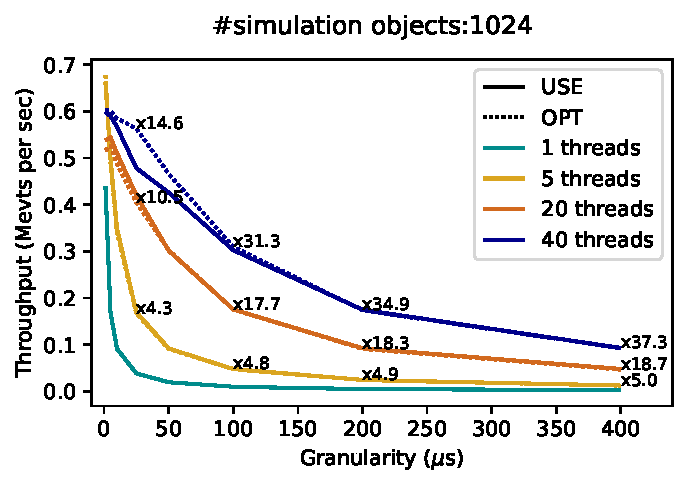
\includegraphics[width=\linewidth]{figures_original/figure7-v2.pdf}
\renewcommand{\thesubfigure}{Original}
\caption{}
\end{subfigure}
\hspace{1cm}
\begin{subfigure}[b]{\mysize}
\centering
\IfFileExists{data/figure7.csv}{
  \IfFileExists{figures_reproduced/figure8.pdf}{
\includegraphics[width=\linewidth]{figures_reproduced/figure8.pdf}
  }{\texttt{figures\_reproduced/figure8.pdf} not found and \texttt{figure7.csv} found, please re-run \texttt{./process\_data.sh 07\_and\_08} first and then contact contributors}
}{\texttt{data/figure7.csv} not found, please run \texttt{./process\_data.sh 07\_and\_08} first}
\renewcommand{\thesubfigure}{Reproduced}
\caption{}
\end{subfigure}
\caption{Throughput of PHOLD  with different event granularities and thread counts. Each label represents the speedup relative to the sequential execution for a given event granularity and thread count.}
\end{figure}

\clearpage


\section*{Figure 9}

%%%%%%%%%%%%%%%%%%%%%%%%%%%%%%%%%%%%%%%%%%%%%%%%
%  FIGURE 9a
%%%%%%%%%%%%%%%%%%%%%%%%%%%%%%%%%%%%%%%%%%%%%%%%


\renewcommand{\mysize}{0.7\linewidth}

\setcounter{figure}{8}
\renewcommand{\thefigure}{\arabic{figure}a}
\begin{figure}[!h]
\centering
\begin{subfigure}[b]{\mysize}
\centering
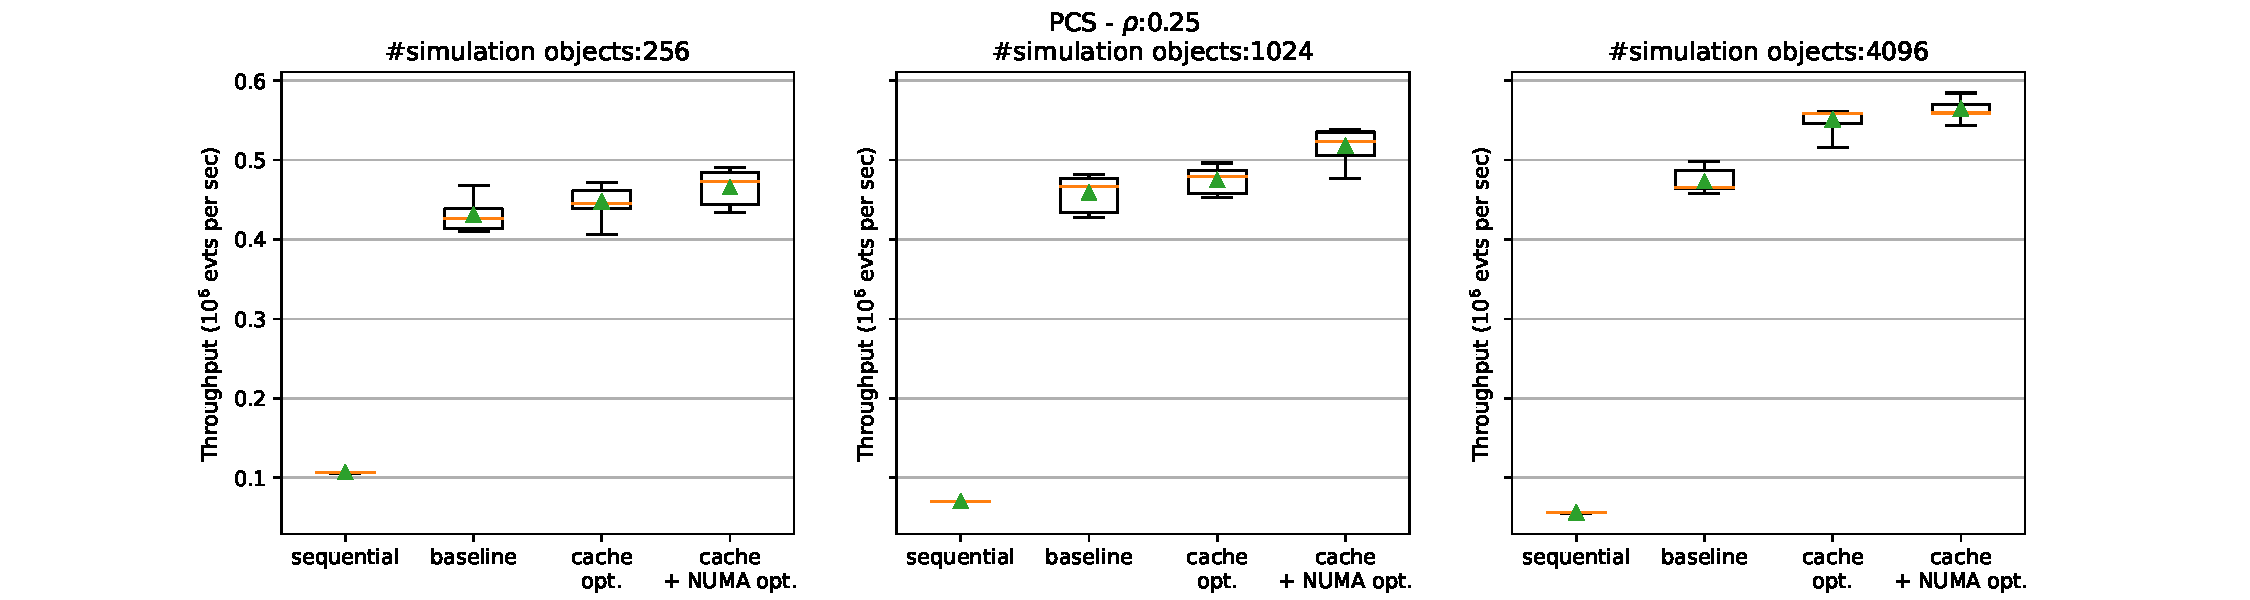
\includegraphics[width=0.85\textwidth, clip, trim=80 0 80 0]{figures_original/results-pcs-0.48-pcs-half.pdf}
\renewcommand{\thesubfigure}{Original}
\caption{}
\end{subfigure}
\begin{subfigure}[b]{\mysize}
\centering
\IfFileExists{figures_reproduced/figure9a-results-pcs-0.48-pcs-half.pdf}{
\includegraphics[width=0.85\textwidth, clip, trim=80 0 80 0]{figures_reproduced/figure9a-results-pcs-0.48-pcs-half.pdf}
}{\texttt{figures\_reproduced/figure9a-results-pcs-0.48-pcs-half.pdf} not found, please run \texttt{./process\_data.sh 09} first}
\renewcommand{\thesubfigure}{Reproduced}
\caption{}
\end{subfigure}
\caption{Results with PCS. --- Execution speed with $\rho=0.25$.}% with different utilization factors of channels.}
\end{figure}


%%%%%%%%%%%%%%%%%%%%%%%%%%%%%%%%%%%%%%%%%%%%%%%%
%  FIGURE 9b
%%%%%%%%%%%%%%%%%%%%%%%%%%%%%%%%%%%%%%%%%%%%%%%%

\setcounter{figure}{8}
\renewcommand{\thefigure}{\arabic{figure}b}
\begin{figure}[!h]
\centering
\begin{subfigure}[b]{\mysize}
\centering
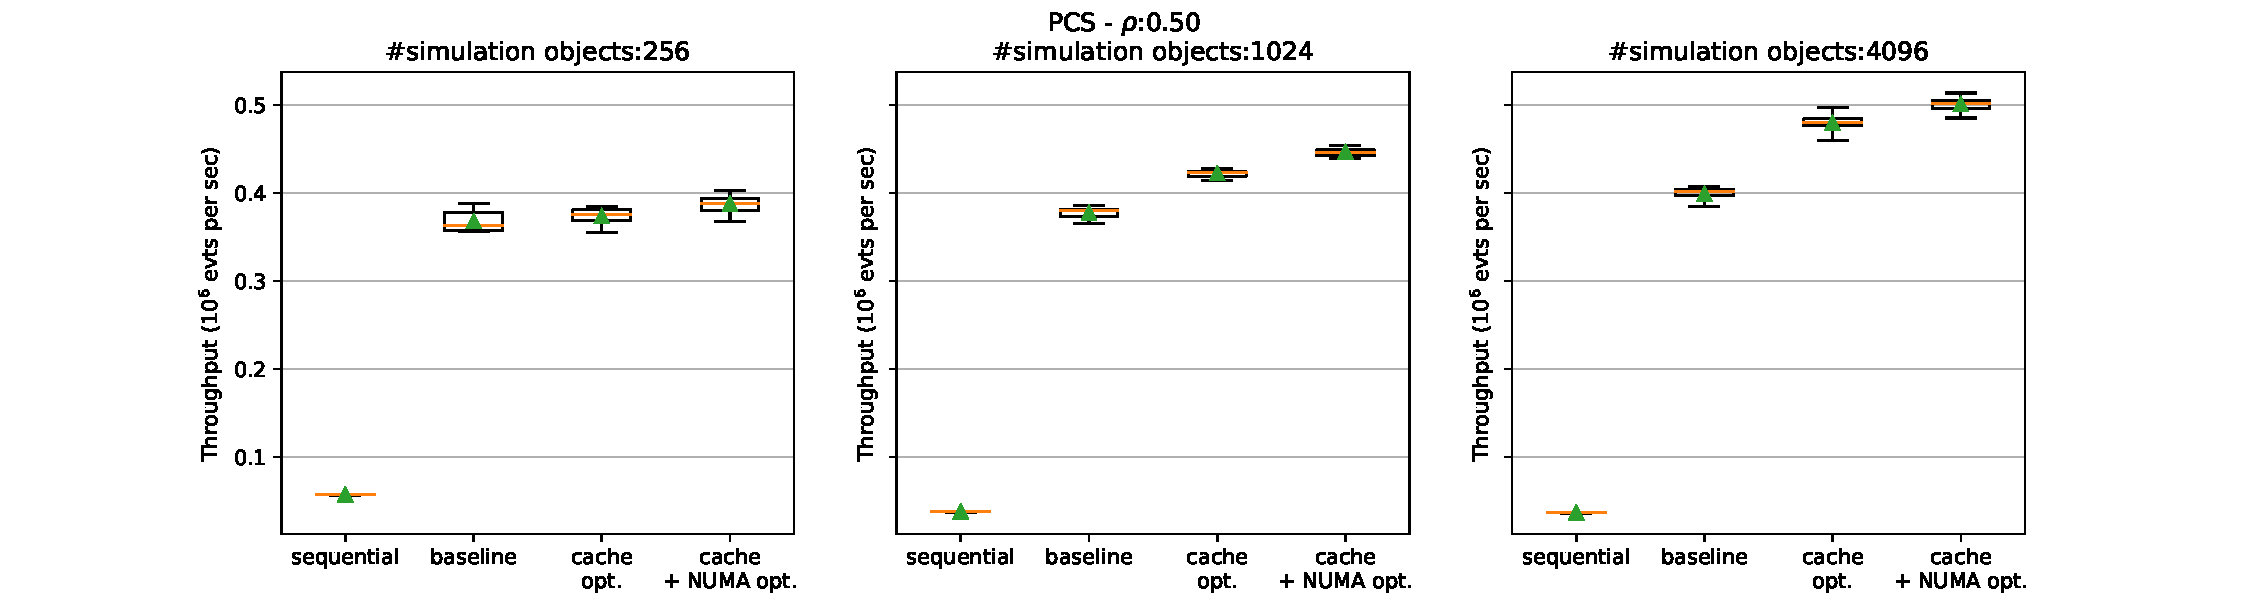
\includegraphics[width=0.85\textwidth, clip, trim=80 0 80 0]{figures_original/results-pcs-0.24-pcs-half.pdf}
\renewcommand{\thesubfigure}{Original}
\caption{}
\end{subfigure}
\begin{subfigure}[b]{\mysize}
\centering
\IfFileExists{figures_reproduced/figure9b-results-pcs-0.24-pcs-half.pdf}{
\includegraphics[width=0.85\textwidth, clip, trim=80 0 80 0]{figures_reproduced/figure9b-results-pcs-0.24-pcs-half.pdf}
}{\texttt{figures\_reproduced/figure9b-results-pcs-0.24-pcs-half.pdf} not found, please run \texttt{./process\_data.sh 09} first}
\renewcommand{\thesubfigure}{Reproduced}
\caption{}
\end{subfigure}
\caption{Results with PCS. --- Execution speed with $\rho=0.5$.}% with different utilization factors of channels.}
\end{figure}

%%%%%%%%%%%%%%%%%%%%%%%%%%%%%%%%%%%%%%%%%%%%%%%%
%  FIGURE 9c
%%%%%%%%%%%%%%%%%%%%%%%%%%%%%%%%%%%%%%%%%%%%%%%%

\newpage

\setcounter{figure}{8}
\renewcommand{\thefigure}{\arabic{figure}c}
\begin{figure}[!h]
\centering
\begin{subfigure}[b]{\mysize}
\centering
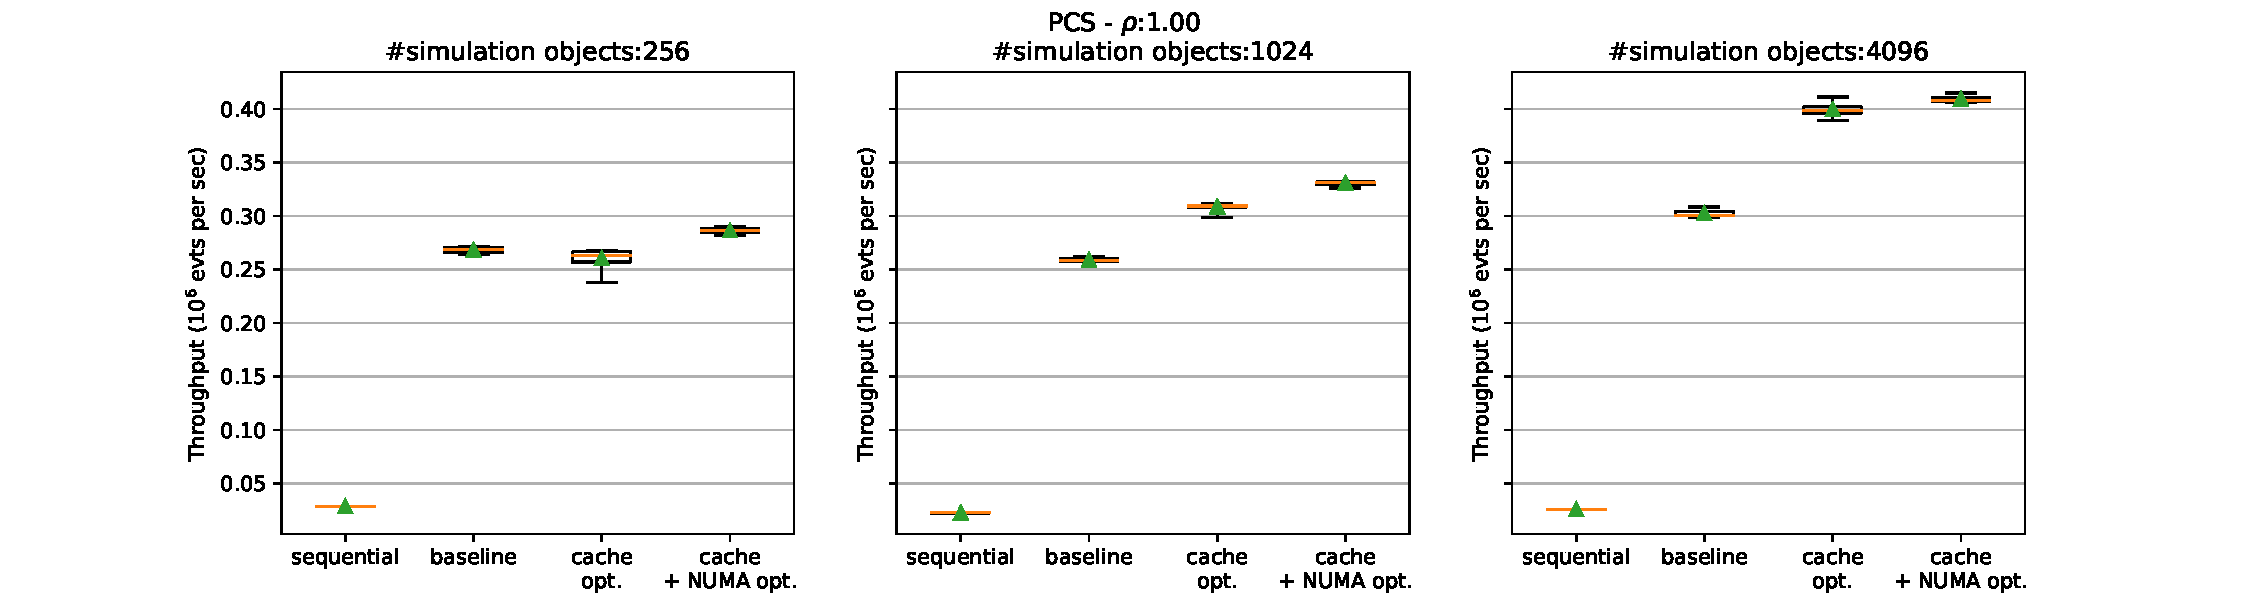
\includegraphics[width=0.85\textwidth, clip, trim=80 0 80 0]{figures_original/results-pcs-0.12-pcs-half.pdf}
\renewcommand{\thesubfigure}{Original}
\caption{}
\end{subfigure}
\begin{subfigure}[b]{\mysize}
\centering
\IfFileExists{figures_reproduced/figure9c-results-pcs-0.12-pcs-half.pdf}{
\includegraphics[width=0.85\textwidth, clip, trim=80 0 80 0]{figures_reproduced/figure9c-results-pcs-0.12-pcs-half.pdf}
}{\texttt{figures\_reproduced/figure9c-results-pcs-0.12-pcs-half.pdf} not found, please run \texttt{./process\_data.sh 09} first}
\renewcommand{\thesubfigure}{Reproduced}
\caption{}
\end{subfigure}
\caption{Results with PCS. --- Execution speed with $\rho=1.0$.}% with different utilization factors of channels.}
\end{figure}





%%%%%%%%%%%%%%%%%%%%%%%%%%%%%%%%%%%%%%%%%%%%%%%%
%  Table 2
%%%%%%%%%%%%%%%%%%%%%%%%%%%%%%%%%%%%%%%%%%%%%%%%

\section*{Table 2}

\setcounter{table}{1}
\renewcommand{\thetable}{\arabic{table} Original}
\begin{table}[!h]
\footnotesize \centering
\caption{Average rollback frequency}
\begin{tabular}{r||c|c|c||c|c|c||c|c|c}
{\sc Utilization factor}  & \multicolumn{3}{c||}{$\rho$ = $0.25$}  & \multicolumn{3}{c||}{$\rho$ = $0.50$}  & \multicolumn{3}{c}{$\rho$  = $1.00$} \\ \hline
{\sc \#Simulation objects} & 256 & 1024 & 4096 & 256 & 1024 & 4096 & 256 & 1024 & 4096 \\ \hline \hline
%\multirow{3}{*}{\sc Version }
{\bf baseline}             &       0.71\% &       0.19\% &       0.05\% &       0.77\% &       0.22\% &       0.05\% &       0.91\% &       0.24\% &       0.05\% \\ \hline
{\bf cache opt.}          &       2.12\% &       2.68\% &       3.21\% &       2.80\% &       3.29\% &       2.94\% &       2.81\% &       3.24\% &       2.55\% \\ \hline
{\bf cache+NUMA opt.}    &       2.62\% &       3.14\% &       3.16\% &       2.75\% &       3.49\% &       3.03\% &       2.95\% &       3.28\% &       2.64\%
\end{tabular}
\end{table}

\setcounter{table}{1}
\renewcommand{\thetable}{\arabic{table} Reproduced}
\begin{table}[!h]
\footnotesize \centering
\caption{Average rollback frequency}
\begin{tabular}{r||c|c|c||c|c|c||c|c|c}
{\sc Utilization factor}  & \multicolumn{3}{c||}{$\rho$ = $0.25$}  & \multicolumn{3}{c||}{$\rho$ = $0.50$}  & \multicolumn{3}{c}{$\rho$  = $1.00$} \\ \hline
{\sc \#Simulation objects} & 256 & 1024 & 4096 & 256 & 1024 & 4096 & 256 & 1024 & 4096 \\ \hline \hline
\IfFileExists{figures_reproduced/table2.tex}{
\input{figures_reproduced/table2.tex}
}{\texttt{figures\_reproduced/table2.tex} not found, please run \texttt{./process\_data.sh 09} first}
\end{tabular}
\end{table}



%%%%%%%%%%%%%%%%%%%%%%%%%%%%%%%%%%%%%%%%%%%%%%%%
%  Table 3
%%%%%%%%%%%%%%%%%%%%%%%%%%%%%%%%%%%%%%%%%%%%%%%%


\section*{Table 3}

\setcounter{table}{2}
\renewcommand{\thetable}{\arabic{table} Original}
\begin{table}[!h]
\footnotesize \centering
\caption{Average rollback length}
\label{ta:pcsrollbackslen}
\begin{tabular}{r||c|c|c||c|c|c||c|c|c}
  {\sc Utilization factor}  & \multicolumn{3}{c||}{$\rho$ = $0.25$}  & \multicolumn{3}{c||}{$\rho$ = $0.50$}  & \multicolumn{3}{c}{$\rho$  = $1.00$} \\ \hline
  {\sc \#Simulation objects} & 256 & 1024 & 4096 & 256 & 1024 & 4096 & 256 & 1024 & 4096 \\ \hline \hline

{\bf baseline}  & 1.06   & 1.02   & 1.01   & 1.08   & 1.02   & 1.01   & 1.08   & 1.02   & 1.01   \\ \hline
{\bf cache opt.} & 1.97   & 2.55   & 3.84   & 2.06   & 3.55   & 4.14   & 2.13   & 4.01   & 5.08   \\ \hline
{\bf cache+NUMA opt.} & 2.08   & 2.50   & 4.04   & 1.99   & 3.25   & 3.97   & 2.06   & 3.34   & 5.01   \\ \hline
\end{tabular}
\end{table}

\setcounter{table}{2}
\renewcommand{\thetable}{\arabic{table} Reproduced}
\begin{table}[!h]
\footnotesize \centering
\caption{Average rollback length}
\label{ta:pcsrollbackslen}
\begin{tabular}{r||c|c|c||c|c|c||c|c|c}
{\sc Utilization factor}  & \multicolumn{3}{c||}{$\rho$ = $0.25$}  & \multicolumn{3}{c||}{$\rho$ = $0.50$}  & \multicolumn{3}{c}{$\rho$  = $1.00$} \\ \hline
{\sc \#Simulation objects} & 256 & 1024 & 4096 & 256 & 1024 & 4096 & 256 & 1024 & 4096 \\ \hline \hline
\IfFileExists{figures_reproduced/table3.tex}{
\input{figures_reproduced/table3.tex}
}{\texttt{figures\_reproduced/table3.tex} not found, please run \texttt{./process\_data.sh 09} first}

\end{tabular}
\end{table}



\newpage



%%%%%%%%%%%%%%%%%%%%%%%%%%%%%%%%%%%%%%%%%%%%%%%%
%  FIGURE 10a
%%%%%%%%%%%%%%%%%%%%%%%%%%%%%%%%%%%%%%%%%%%%%%%%


\section*{Figure 10}

\setcounter{figure}{9}
\renewcommand{\thefigure}{\arabic{figure}a}
\renewcommand{\mysize}{0.2\linewidth}

\begin{figure}[!h]
\centering
\begin{subfigure}[b]{\mysize}
\centering
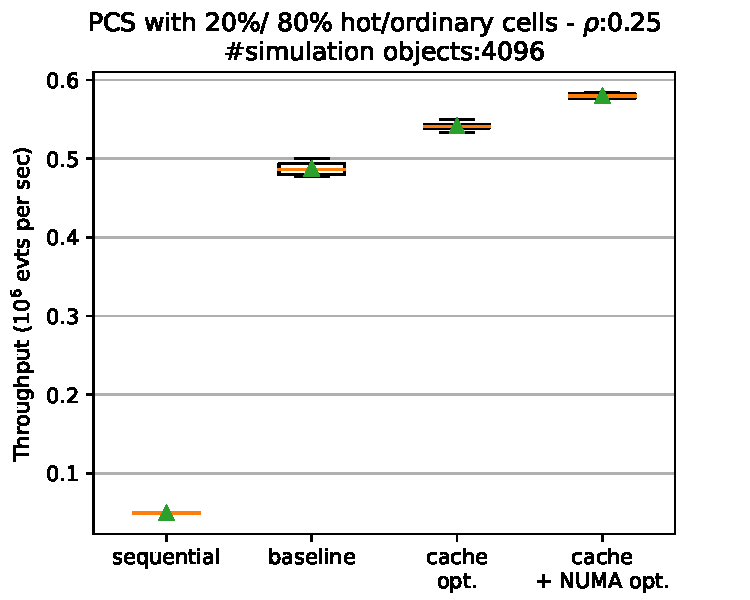
\includegraphics[width=\linewidth]{figures_original/results-pcs-hs-0.48-pcs_hs-half.pdf}
\renewcommand{\thesubfigure}{Original}
\caption{}
\end{subfigure}
\begin{subfigure}[b]{\mysize}
\centering
\IfFileExists{figures_reproduced/figure10a-results-pcs-hs-0.48-pcs_hs-half.pdf}{
\includegraphics[width=\linewidth]{figures_reproduced/figure10a-results-pcs-hs-0.48-pcs_hs-half.pdf}
}{\texttt{figures\_reproduced/figure10a-results-pcs-hs-0.48-pcs\_hs-half.pdf} not found, please run \texttt{./process\_data.sh 10} first}
\renewcommand{\thesubfigure}{Reproduced}
\caption{}
\end{subfigure}
\caption{Results with PCS with 20\% of hot-spot cells. --- Execution speed.}
\end{figure}


%%%%%%%%%%%%%%%%%%%%%%%%%%%%%%%%%%%%%%%%%%%%%%%%
%  FIGURE 10b
%%%%%%%%%%%%%%%%%%%%%%%%%%%%%%%%%%%%%%%%%%%%%%%%




\setcounter{figure}{9}
\renewcommand{\thefigure}{\arabic{figure}b}
\renewcommand{\mysize}{0.2\linewidth}

\begin{figure}[!h]
\centering
\begin{subfigure}[b]{\mysize}
\centering
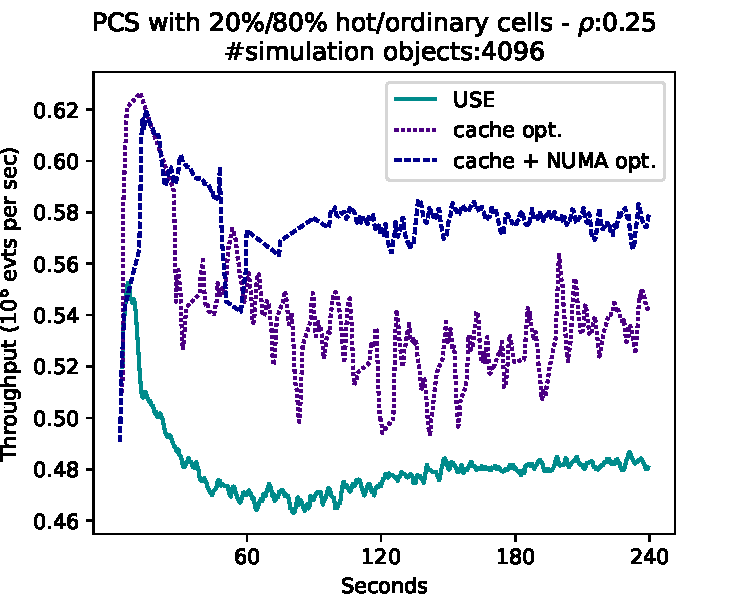
\includegraphics[width=\linewidth]{figures_original/results-pcs-hs-0.48-pcs_hs-240-1.pdf}
\renewcommand{\thesubfigure}{Original}
\caption{}
\end{subfigure}


\IfFileExists{figures_reproduced/figure10b-results-pcs-hs-0.48-pcs_hs-240-0.pdf}{
\begin{subfigure}[b]{\mysize}
\centering
\includegraphics[width=\textwidth]{figures_reproduced/figure10b-results-pcs-hs-0.48-pcs_hs-240-0.pdf}    
\renewcommand{\thesubfigure}{Reproduced 1}
\caption{}
\end{subfigure}
\begin{subfigure}[b]{\mysize}
\centering
\includegraphics[width=\textwidth]{figures_reproduced/figure10b-results-pcs-hs-0.48-pcs_hs-240-1.pdf}    
\renewcommand{\thesubfigure}{Reproduced 2}
\caption{}
\end{subfigure}
\begin{subfigure}[b]{\mysize}
\centering
\includegraphics[width=\textwidth]{figures_reproduced/figure10b-results-pcs-hs-0.48-pcs_hs-240-2.pdf}    
\renewcommand{\thesubfigure}{Reproduced 3}
\caption{}
\end{subfigure}
\begin{subfigure}[b]{\mysize}
\centering
\includegraphics[width=\textwidth]{figures_reproduced/figure10b-results-pcs-hs-0.48-pcs_hs-240-3.pdf}    
\renewcommand{\thesubfigure}{Reproduced 4}
\caption{}
\end{subfigure}
\begin{subfigure}[b]{\mysize}
\centering
\includegraphics[width=\textwidth]{figures_reproduced/figure10b-results-pcs-hs-0.48-pcs_hs-240-4.pdf}    
\renewcommand{\thesubfigure}{Reproduced 5}
\caption{}
\end{subfigure}
\begin{subfigure}[b]{\mysize}
\centering
\includegraphics[width=\textwidth]{figures_reproduced/figure10b-results-pcs-hs-0.48-pcs_hs-240-5.pdf}    
\renewcommand{\thesubfigure}{Reproduced 6}
\caption{}
\end{subfigure}
}{
\begin{subfigure}[b]{\mysize}
\centering
\texttt{figures\_reproduced/figure10b-results-pcs-hs-0.48-pcs\_hs-240-*.pdf} not found, please run \texttt{./process\_data.sh 10} first
\renewcommand{\thesubfigure}{Reproduced}
\caption{}
\end{subfigure}
}
\caption{Results with PCS with 20\% of hot-spot cells. --- Execution speed.}
\end{figure}

\section*{Figure 11}

%%%%%%%%%%%%%%%%%%%%%%%%%%%%%%%%%%%%%%%%%%%%%%%%
%  FIGURE 11a
%%%%%%%%%%%%%%%%%%%%%%%%%%%%%%%%%%%%%%%%%%%%%%%%

\setcounter{figure}{10}
\renewcommand{\thefigure}{\arabic{figure}a}
\renewcommand{\mysize}{0.2\linewidth}

\begin{figure}[!h]
\centering
\begin{subfigure}[b]{\mysize}
\centering
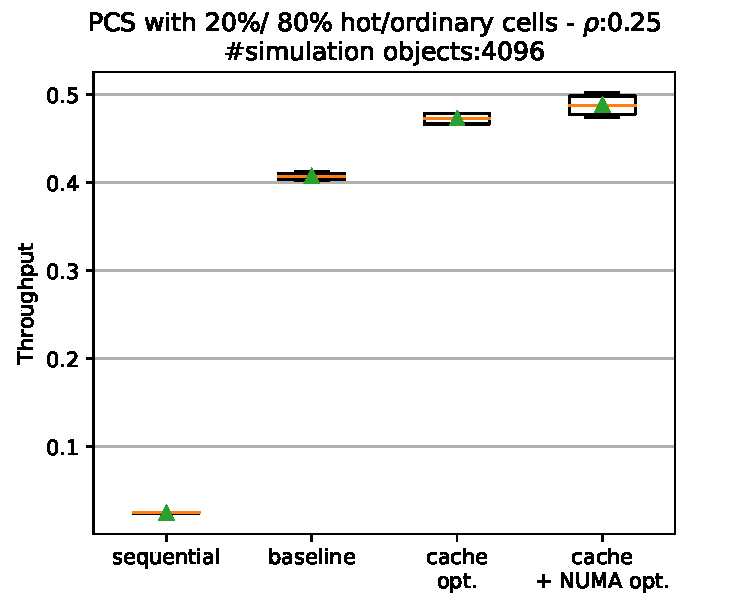
\includegraphics[width=\linewidth]{figures_original/results-pcs-dyn-0.48-pcs_hs-half.pdf}
\renewcommand{\thesubfigure}{Original}
\caption{}
\end{subfigure}
\begin{subfigure}[b]{\mysize}
\centering
\IfFileExists{figures_reproduced/figure11a-results-pcs-dynho-pcs_hs_dyn-half.pdf}{
\includegraphics[width=\linewidth]{figures_reproduced/figure11a-results-pcs-dynho-pcs_hs_dyn-half.pdf}
}{\texttt{figures\_reproduced/figure11a-results-pcs-dynho-pcs\_hs\_dyn-half.pdf} not found, please run \texttt{./process\_data.sh 11} first}
\renewcommand{\thesubfigure}{Reproduced}
\caption{}
\end{subfigure}
\caption{Results with PCS with moving 20\% of hot-spot cells. --- Execution speed.}
\end{figure}

\clearpage


%%%%%%%%%%%%%%%%%%%%%%%%%%%%%%%%%%%%%%%%%%%%%%%%
%  FIGURE 11b
%%%%%%%%%%%%%%%%%%%%%%%%%%%%%%%%%%%%%%%%%%%%%%%%



\setcounter{figure}{10}
\renewcommand{\thefigure}{\arabic{figure}b}
\renewcommand{\mysize}{0.2\linewidth}

\begin{figure}[!h]
\centering
\begin{subfigure}[b]{\mysize}
\centering
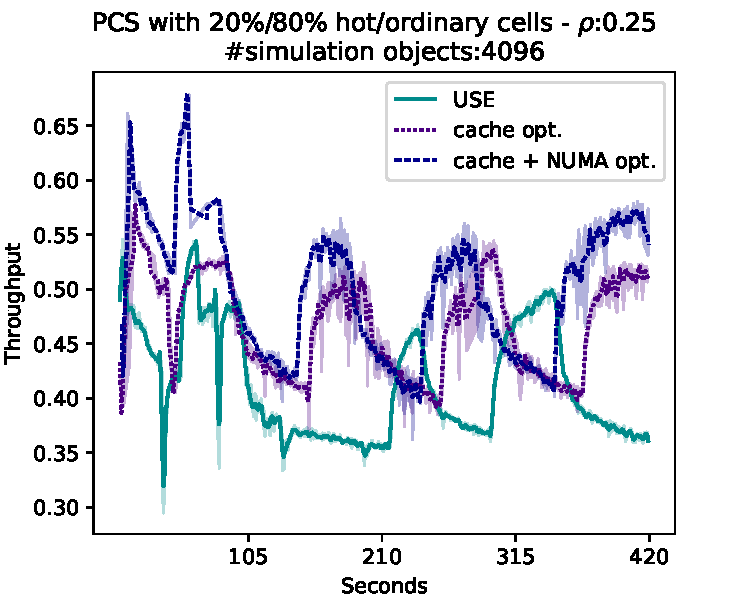
\includegraphics[width=\linewidth]{figures_original/results-pcs-dyn-0.48-pcs_hs-420-0.pdf}
\renewcommand{\thesubfigure}{Original}
\caption{}
\end{subfigure}

\IfFileExists{figures_reproduced/figure11a-results-pcs-dynho-pcs_hs_dyn-half.pdf}{
\begin{subfigure}[b]{\mysize}
\centering
\includegraphics[width=\textwidth]{figures_reproduced/figure11b-results-pcs-dynho-pcs_hs_dyn-420-0.pdf}    
\renewcommand{\thesubfigure}{Reproduced 1}
\caption{}
\end{subfigure}
\begin{subfigure}[b]{\mysize}
\centering
\includegraphics[width=\textwidth]{figures_reproduced/figure11b-results-pcs-dynho-pcs_hs_dyn-420-1.pdf}    
\renewcommand{\thesubfigure}{Reproduced 2}
\caption{}
\end{subfigure}
\begin{subfigure}[b]{\mysize}
\centering
\includegraphics[width=\textwidth]{figures_reproduced/figure11b-results-pcs-dynho-pcs_hs_dyn-420-2.pdf}    
\renewcommand{\thesubfigure}{Reproduced 3}
\caption{}
\end{subfigure}
\begin{subfigure}[b]{\mysize}
\centering
\includegraphics[width=\textwidth]{figures_reproduced/figure11b-results-pcs-dynho-pcs_hs_dyn-420-3.pdf}    
\renewcommand{\thesubfigure}{Reproduced 4}
\caption{}
\end{subfigure}
\begin{subfigure}[b]{\mysize}
\centering
\includegraphics[width=\textwidth]{figures_reproduced/figure11b-results-pcs-dynho-pcs_hs_dyn-420-4.pdf}    
\renewcommand{\thesubfigure}{Reproduced 5}
\caption{}
\end{subfigure}
\begin{subfigure}[b]{\mysize}
\centering
\includegraphics[width=\textwidth]{figures_reproduced/figure11b-results-pcs-dynho-pcs_hs_dyn-420-5.pdf}    
\renewcommand{\thesubfigure}{Reproduced 6}
\caption{}
\end{subfigure}
}
{
\begin{subfigure}[b]{\mysize}
\centering
\texttt{figures\_reproduced/figure11b-results-pcs-dynho-pcs\_hs\_dyn-420-*.pdf} not found, please run \texttt{./process\_data.sh 11} first
\renewcommand{\thesubfigure}{Reproduced 6}
\caption{}
\end{subfigure}
}
\caption{Results with PCS with 20\% of hot-spot cells. --- Event throughput for an individual simulation run.}
\end{figure}



%%%%%%%%%%%%%%%%%%%%%%%%%%%%%%%%%%%%%%%%%%%%%%%%
%  FIGURE 11c
%%%%%%%%%%%%%%%%%%%%%%%%%%%%%%%%%%%%%%%%%%%%%%%%



\setcounter{figure}{10}
\renewcommand{\thefigure}{\arabic{figure}c}
\renewcommand{\mysize}{0.2\linewidth}

\begin{figure}[!h]
\centering
\begin{subfigure}[b]{\mysize}
\centering
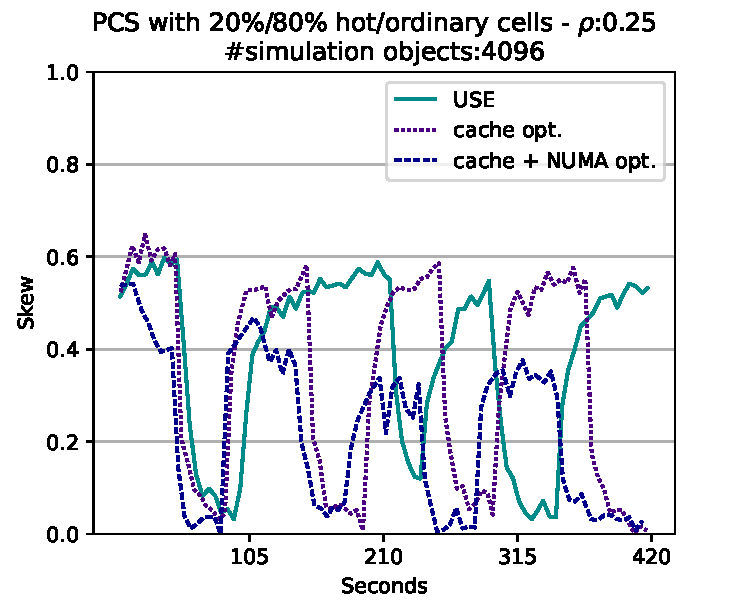
\includegraphics[width=\linewidth]{figures_original/results-pcs-dyn-0.48-pcs_hs-420-0-skew.pdf}
\renewcommand{\thesubfigure}{Original}
\caption{}
\end{subfigure}

\IfFileExists{figures_reproduced/figure11c-results-pcs-dynho-pcs_hs_dyn-420-skew-0.pdf}{
\begin{subfigure}[b]{\mysize}
\centering
\includegraphics[width=\textwidth]{figures_reproduced/figure11c-results-pcs-dynho-pcs_hs_dyn-420-skew-0.pdf}    
\renewcommand{\thesubfigure}{Reproduced 1}
\caption{}
\end{subfigure}
\begin{subfigure}[b]{\mysize}
\centering
\includegraphics[width=\textwidth]{figures_reproduced/figure11c-results-pcs-dynho-pcs_hs_dyn-420-skew-1.pdf}    
\renewcommand{\thesubfigure}{Reproduced 2}
\caption{}
\end{subfigure}
\begin{subfigure}[b]{\mysize}
\centering
\includegraphics[width=\textwidth]{figures_reproduced/figure11c-results-pcs-dynho-pcs_hs_dyn-420-skew-2.pdf}    
\renewcommand{\thesubfigure}{Reproduced 3}
\caption{}
\end{subfigure}
\begin{subfigure}[b]{\mysize}
\centering
\includegraphics[width=\textwidth]{figures_reproduced/figure11c-results-pcs-dynho-pcs_hs_dyn-420-skew-3.pdf}    
\renewcommand{\thesubfigure}{Reproduced 4}
\caption{}
\end{subfigure}
\begin{subfigure}[b]{\mysize}
\centering
\includegraphics[width=\textwidth]{figures_reproduced/figure11c-results-pcs-dynho-pcs_hs_dyn-420-skew-4.pdf}    
\renewcommand{\thesubfigure}{Reproduced 5}
\caption{}
\end{subfigure}
\begin{subfigure}[b]{\mysize}
\centering
\includegraphics[width=\textwidth]{figures_reproduced/figure11c-results-pcs-dynho-pcs_hs_dyn-420-skew-5.pdf}    
\renewcommand{\thesubfigure}{Reproduced 6}
\caption{}
\end{subfigure}

}
{
\begin{subfigure}[b]{\mysize}
\centering
\texttt{figures\_reproduced/figure11c-results-pcs-dynho-pcs\_hs\_dyn-420-skew-*.pdf} not found, please run \texttt{./process\_data.sh 11} first
\renewcommand{\thesubfigure}{Reproduced 6}
\caption{}
\end{subfigure}
}

\caption{Results with PCS with 20\% of hot-spot cells. --- Workload skew between the two NUMA nodes.}
\end{figure}



%%%%%%%%%%%%%%%%%%%%%%%%%%%%%%%%%%%%%%%%%%%%%%%%
%  FIGURE 11d
%%%%%%%%%%%%%%%%%%%%%%%%%%%%%%%%%%%%%%%%%%%%%%%%



\setcounter{figure}{10}
\renewcommand{\thefigure}{\arabic{figure}d}
\renewcommand{\mysize}{0.2\linewidth}

\begin{figure}[!h]
\centering
\begin{subfigure}[b]{\mysize}
\centering
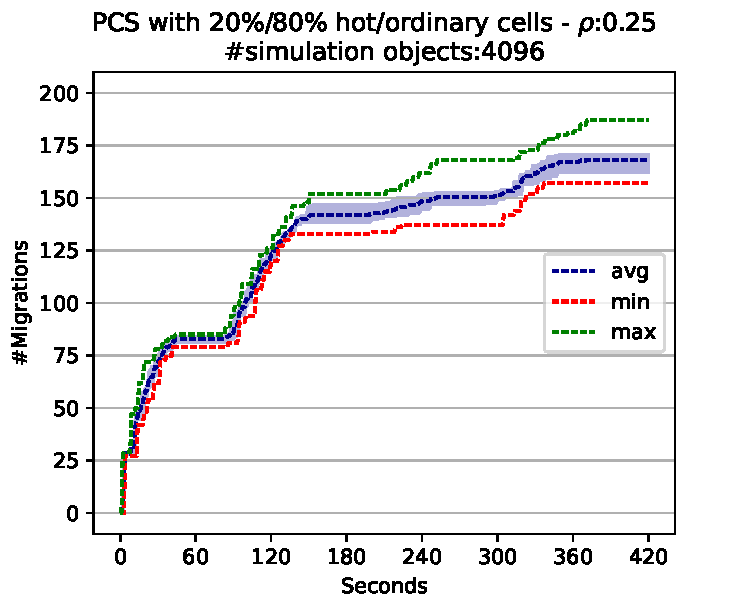
\includegraphics[width=\linewidth]{figures_original/results-pcs-dyn-0.48-pcs_hs-420-mcnt.pdf}
\renewcommand{\thesubfigure}{Original}
\caption{}
\end{subfigure}
\begin{subfigure}[b]{\mysize}
\centering
\IfFileExists{figures_reproduced/figure11d-results-pcs-dynho-pcs_hs-420-mcnt.pdf}{
\includegraphics[width=\textwidth]{figures_reproduced/figure11d-results-pcs-dynho-pcs_hs-420-mcnt.pdf}
}{\texttt{figures\_reproduced/figure11d-results-pcs-dynho-pcs\_hs-420-mcnt.pdf} not found, please run \texttt{./process\_data.sh 11} first}
\renewcommand{\thesubfigure}{Reproduced}
\caption{}
\end{subfigure}
\caption{Results with PCS with moving 20\% of hot-spot cells. --- Average cumulative number of migrations.}
\end{figure}



\clearpage
%%%%%%%%%%%%%%%%%%%%%%%%%%%%%%%%%%%%%%%%%%%%%%%%
%  FIGURE 12
%%%%%%%%%%%%%%%%%%%%%%%%%%%%%%%%%%%%%%%%%%%%%%%%
{}~{}\newline
\section*{Figure 12}
\renewcommand{\thefigure}{\arabic{figure}}
\renewcommand{\mysize}{0.2\linewidth}
\begin{figure}[!h]
\centering
\begin{subfigure}[b]{\mysize}
\centering
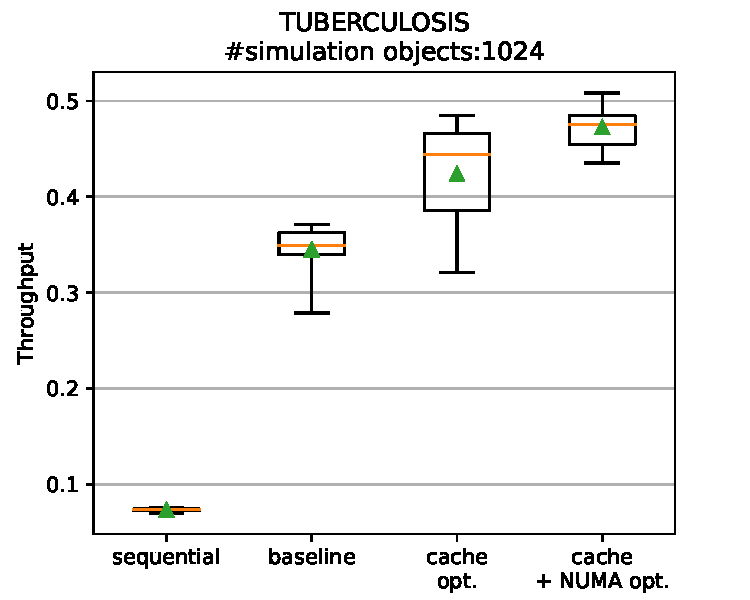
\includegraphics[width=\linewidth]{figures_original/results-results_tuberculosis-tuberculosis-9 .pdf}
\renewcommand{\thesubfigure}{Original}
\caption{}
\end{subfigure}
\begin{subfigure}[b]{\mysize}
\centering
\IfFileExists{figures_reproduced/figure12-results-results_tuberculosis-tuberculosis-9 .pdf}{
\includegraphics[width=\textwidth]{figures_reproduced/figure12-results-results_tuberculosis-tuberculosis-9 .pdf}
}{\texttt{figures\_reproduced/figure12-results-results\_tuberculosis-tuberculosis-9 .pdf} not found, please run \texttt{./process\_data.sh 12} first}
\renewcommand{\thesubfigure}{Reproduced}
\caption{}
\end{subfigure}
\caption{TBC execution speed}
\end{figure}


%%%%%%%%%%%%%%%%%%%%%%%%%%%%%%%%%%%%%%%%%%%%%%%%
%  Table 4
%%%%%%%%%%%%%%%%%%%%%%%%%%%%%%%%%%%%%%%%%%%%%%%%


\section*{Table 4}


\setcounter{table}{3}
\renewcommand{\thetable}{\arabic{table} Original}
\begin{table}[!h]
\footnotesize \centering
\caption{Average rollback frequency}
\begin{tabular}{r|c}
{\bf baseline} & 0.0010\%  \\ \hline
{\bf cache opt.} & 1.5610\%  \\ \hline
{\bf cache+NUMA opt.} & 1.6323\%  \\
\end{tabular}
\end{table}


\setcounter{table}{3}
\renewcommand{\thetable}{\arabic{table} Reproduced}
\begin{table}[!h]
\footnotesize \centering
\caption{Average rollback frequency}
\begin{tabular}{r|c}
\IfFileExists{figures_reproduced/table4.tex}{
\input{figures_reproduced/table4.tex}
}{\texttt{figures\_reproduced/table4.tex} not found, please run \texttt{./process\_data.sh 09} first}
\end{tabular}
\end{table}


%%%%%%%%%%%%%%%%%%%%%%%%%%%%%%%%%%%%%%%%%%%%%%%%
%  Table 5
%%%%%%%%%%%%%%%%%%%%%%%%%%%%%%%%%%%%%%%%%%%%%%%%


\section*{Table 5}

\setcounter{table}{4}
\renewcommand{\thetable}{\arabic{table} Original}
\begin{table}[!h]
\footnotesize \centering
\caption{Average rollback length}
\begin{tabular}{r|c}
{\bf baseline} & 1.13  \\ \hline
{\bf cache opt.} & 1.51  \\ \hline
{\bf cache + NUMA opt.} & 1.57  \\
\end{tabular}
\end{table}

\setcounter{table}{4}
\renewcommand{\thetable}{\arabic{table} Reproduced}
\begin{table}[!h]
\footnotesize \centering
\caption{Average rollback length}
\begin{tabular}{r|c}
\IfFileExists{figures_reproduced/table5.tex}{
\input{figures_reproduced/table5.tex}
}{\texttt{figures\_reproduced/table5.tex} not found, please run \texttt{./process\_data.sh 09} first}
\end{tabular}
\end{table}

\end{document}
